\documentclass[10pt]{report}

\usepackage{talks}
\newcommand{\expect}[1]{\mathbb{E}\!\left[ #1 \right]}
\newcommand{\reals}{\mathbb{R}}
\newcommand{\draw}[2]{#1^{(#2)}}
\usepackage{mathpazo}
\usepackage{sourcecodepro}
\usepackage{tikz}
  \usetikzlibrary{arrows.meta, angles, quotes, calc, positioning, shapes}
\renewcommand{\baselinestretch}{1.05}
\newcommand{\ddfrac}[2]{\frac{\strut \displaystyle #1}{\strut \displaystyle #2}}
\newcommand{\pos}[2]{#1^{(#2)}}
    
\begin{document}

\sf
\mbox{ } \\
\spc{\LARGE\bfseries \color{MidnightBlue}{GIST:}}
\\[4pt]
\spc{\Large\bfseries \color{MidnightBlue}{Gibbs self-tuning
    Hamiltonian Monte Carlo}}
\\[12pt]
\noindent 
\spc{\large\bfseries \color{MidnightBlue}{Bob Carpenter}}
\\[2pt]
\spc{\small Center for Computational Mathematics}
\\[-1pt]
\spc{\small Flatiron Institute}
\\[2pt]
\spc{\footnotesize \url{bcarpenter@flatironinstitute.org}}
\\[12pt]
\spc{\small Joint work with Nawaf Bou-Rabee (Rutgers), Milo Marsden
  (Stanford),}
\\
\spc{\small Tore Kleppe (Stavanger), and Edward Roualdes (Cal State)}
\noindent
\\
\vfill
\noindent\spc{\footnotesize June 2024 \qquad University of Trieste}
\hfill

\includegraphics[width=1.25in]{img/flatiron-logo.png}

\sld{Where are we going?}
\begin{itemize}
\item A new \myemph{framework} for
  \myemph{tuning} Hamiltonian Monte Carlo (HMC) samplers
  \begin{subitemize}
    \item (a) \myemph{number of steps}, (b) \myemph{step size}, (c) \myemph{mass matrix}
    \end{subitemize}
\item The \myemph{tuning parameters are Gibbs sampled} conditioned on the
  current position and momentum.
  \begin{subitemize}
  \item may use features of the full trajectories they define.
  \end{subitemize}
\item Metropolis-within-Gibbs \myemph{accept probability adjusted} for balance.
\item \myemph{Non-Markovian warmup} is \myemph{not} required
\begin{subitemize}
\item may still need burnin to find bulk of probability mass
\end{subitemize}
\item We show many popular samplers are instances (e.g., randomized
  HMC, NUTS, multinomial HMC, apogee-to-apogee path sampler)
\end{itemize}

\sld{Bayesian posterior inference is integration}
\begin{itemize}
\item \myemph{Posterior} $p(\theta \mid y) \propto p(y
  \mid \theta) \cdot p(\theta)$ for \myemph{data} $y$, \myemph{parameters} $\theta$
\item \myemph{Parameter estimate} minimizing expected square error:
  $$ \textstyle
  \widehat{\theta}
  = \expect{\theta \mid y}
  = \int_{\mathbb{R}^D}
  \theta \cdot p(\theta \mid y)
  \, \textrm{d}\theta 
  $$
\item \myemph{Event probability} for event $A \subseteq \mathbb{R}^D$:
  $$ \textstyle
  \Pr[A \mid y]
  = \expect{\textrm{I}(\theta \in A) \mid y}
  = \int_{\mathbb{R}^D}
  \textrm{I}(\theta \in A) \cdot p(\theta \mid y) 
  \, \textrm{d}\theta 
  $$
\item \myemph{Posterior predictive density} for new data $\widetilde{y}$:
  $$ \textstyle
  p(\widetilde{y} \mid y) 
  = \expect{p(\widetilde{y} \mid \theta) \mid y}
  = \int_{\mathbb{R}^D}
  p(\widetilde{y} \mid \theta) \cdot p(\theta \mid y) 
  \, \textrm{d}\theta 
  $$
\end{itemize}

\sld{High-dimensional integration is {\slshape Very Hard}}
\begin{itemize}
\item The only general black-box methods are \myemph{Monte Carlo} based.
\item \myemph{Non-gradient methods} (e.g., random-walk Metropolis,
  Gibbs, etc.) 
  scale in dimension as $\mathcal{O}(D^2)$ with \myemph{nasty
    constants} for condition
\item \myemph{Hamiltonian Monte Carlo} (HMC) scales $\mathcal{O}(N^{5/4})$ w.\
  better constants
  \begin{subitemize}
  \item \myemph{order of magnitude} plus improvement in efficiency and
    scalability
  \item with automatic differentiation and probabilistic programming
  \item solid, \myemph{industrial-strength} implementations
  \end{subitemize}
\item HMC is \myemph{notoriously difficult to tune}
  \begin{subitemize}
  \item for \myemph{integration time}, we have NUTS to adapt \myemph{locally}
  \item for \myemph{step size} and \myemph{mass matrix}, we warm up to adapt \myemph{globally}
  \end{subitemize}
\end{itemize}




\sld{Monte Carlo method \hfill {\small (Fermi, Ulam 1930s--1940s)}}
\begin{itemize}
\item Given a Bayesian \myemph{posterior density} $p(\theta \mid y),$
  with support for \myemph{parameters} $\theta \in \mathbb{R}^D$ and \myemph{data} $y$,
  draw a \myemph{sample}
  $$ \textstyle
  \draw{\theta}{1}, \ldots \draw{\theta}{M} \sim p(\theta \mid y)
  $$
\item to evaluate \myemph{posterior expectations} of functions $f$
\begin{align*}
  \textstyle 
  \expect{f(\theta) \mid y}
  &= \textstyle \int_{\mathbb{R}^D} f(\theta) \cdot p(\theta \mid y) \,
    \textrm{d}\theta
  \\[4pt]
  &= \textstyle \lim_{M \rightarrow \infty} \frac{1}{M} \sum_{m=1}^M 
f\left( \draw{\theta}{m} \right)
  \\[4pt] \textstyle
  &\approx \textstyle \frac{1}{M} \sum_{m=1}^M f\left(\draw{\theta}{m}\right) 
\end{align*}
\end{itemize}

\sld{Markov chain Monte Carlo}
\begin{itemize}
\item Usually intractable, if not impossible, to draw an independent sample from a target density.
\item Instead, set up a \myemph{Markov chain} where the \myemph{stationary distribution}
  is the target distribution (i.e., $\theta^{(m)} \sim p(\theta \mid
  y)$ \myemph{marginally})
\item Same \myemph{plug-in estimator} still works with correlated draws.
\item \myemph{MCMC central limit theorem} says \myemph{standard error}
  of estimate is
  $\displaystyle \frac{\textrm{sd}}{\sqrt{\textrm{ESS}}}$,
  \vspace*{-12pt}
  \begin{subitemize}
    \item $\textrm{sd}$ is the \myemph{posterior standard deviation} of the estimand,
    \item and $\textrm{ESS}$ is the \myemph{effective sample size} of the
      sample (as measured in independent draws).
    \item With HMC, effective sample size can exceed sample size
    \end{subitemize}
\end{itemize}



\sld{Fictitious particle Hamiltonian dynamics}
\begin{itemize}
\item \myemph{Auxiliary variable}: couple \myemph{momentum} $\rho \in
  \mathbb{R}^D$ with \myemph{position} $\theta \in \mathbb{R}^D$
\item \myemph{Potential energy}: $U(\theta) = -\log p(\theta \mid y)$
\item \myemph{Kinetic energy}: $K(\rho) = -\log \textrm{normal}(\rho
  \mid 0, \Sigma) = -\frac{1}{2} \cdot \rho^{\top} \cdot \Sigma^{-1} \cdot
  \rho + \textrm{const.}$
\item \myemph{Hamiltonian}: $H(\theta, \rho) = U(\theta) + K(\rho)$
\item \myemph{Dynamics} (time-independent):
  $$
  \nabla_\theta \, H(\theta, \rho) = \rho
  \qquad
  \nabla_\rho \, H(\theta, \rho) = -\nabla_{\theta} \, \log
  p(\theta \mid y)
  $$
\item These ordinary differential equations (ODE) can be \myemph{solved numerically}.
\end{itemize}

\sld{Leapfrog algorithm: $\Phi_{\epsilon, \Sigma}$}
\begin{itemize}
\item \myemph{Explicit solver} for Hamiltonian dynamics.
\item \myemph{Given} log density $\log p(\theta)$, step size
  $\epsilon$, positive definite mass matrix $\Sigma$, 
\item define \myemph{one leapfrog step} $\Phi_{\epsilon, \Sigma}(\theta, \rho) = \theta'', \rho''$, where
  \begin{subitemize}
    \item a. $\rho' = \rho + \nabla \log p(\theta \mid y)$
    \item b. $\theta'' = \theta + \Sigma^{-1} \cdot \rho'$
    \item c. $\rho'' = \rho' + \nabla \log p(\theta' \mid y)$
    \end{subitemize}
\item \myemph{Zero steps} (base): Let $\Phi^0_{\epsilon, \Sigma}$ be the identity function
\item \myemph{One or more steps} (induction): Let $\Phi^{t +
    1}_{\epsilon, \Sigma} = \Phi^t_{\epsilon,\Sigma} \circ
  \Phi_{\epsilon,\Sigma}$
\item \myemph{Leapfrog is stable}: one-step error $\mathcal{O}(\epsilon^3)$, long-range error $\mathcal{O}(\epsilon^2)$
\end{itemize}

\sld{HMC Markov transition}
\begin{itemize}
\item Inputs
  \begin{subitemize}
  \item \myemph{position} $\theta$
  \item \myemph{step size} $\epsilon > 0,$
  \item \myemph{number of steps} $T \in \mathbb{N}$
  \item \myemph{mass matrix} $\Sigma$ (positive definite)
  \end{subitemize}
\item \myemph{Refresh momentum}: Sample $\rho \sim \textrm{normal}(0, \Sigma)$
\item \myemph{Simulate dynamics}:  Let $\theta^*, \rho^* = \Phi_{\epsilon,\Sigma}^T(\theta, \rho)$
\item \myemph{Metropolize}: Return $\theta^*$ if $\textrm{uniform}(0, 1) <
  \frac{\displaystyle p(\theta^*, \rho^*)}
       {\displaystyle p(\theta, \rho)}$ else return $\theta$
\end{itemize}

\sld{Why is HMC hard to tune, even for std.\ normal?}
\begin{subitemize}
  \item HMC (top), randomized steps HMC (bottom); ESS
    $\widehat{\theta}$ (blue) and $\widehat{\theta^2}$ (red); HMC (solid),
    NUTS (dashed); steps (faceted); step size ($x$-axis), ESS ($y$-axis)
\end{subitemize}
\vspace*{-3pt}
\begin{center}
  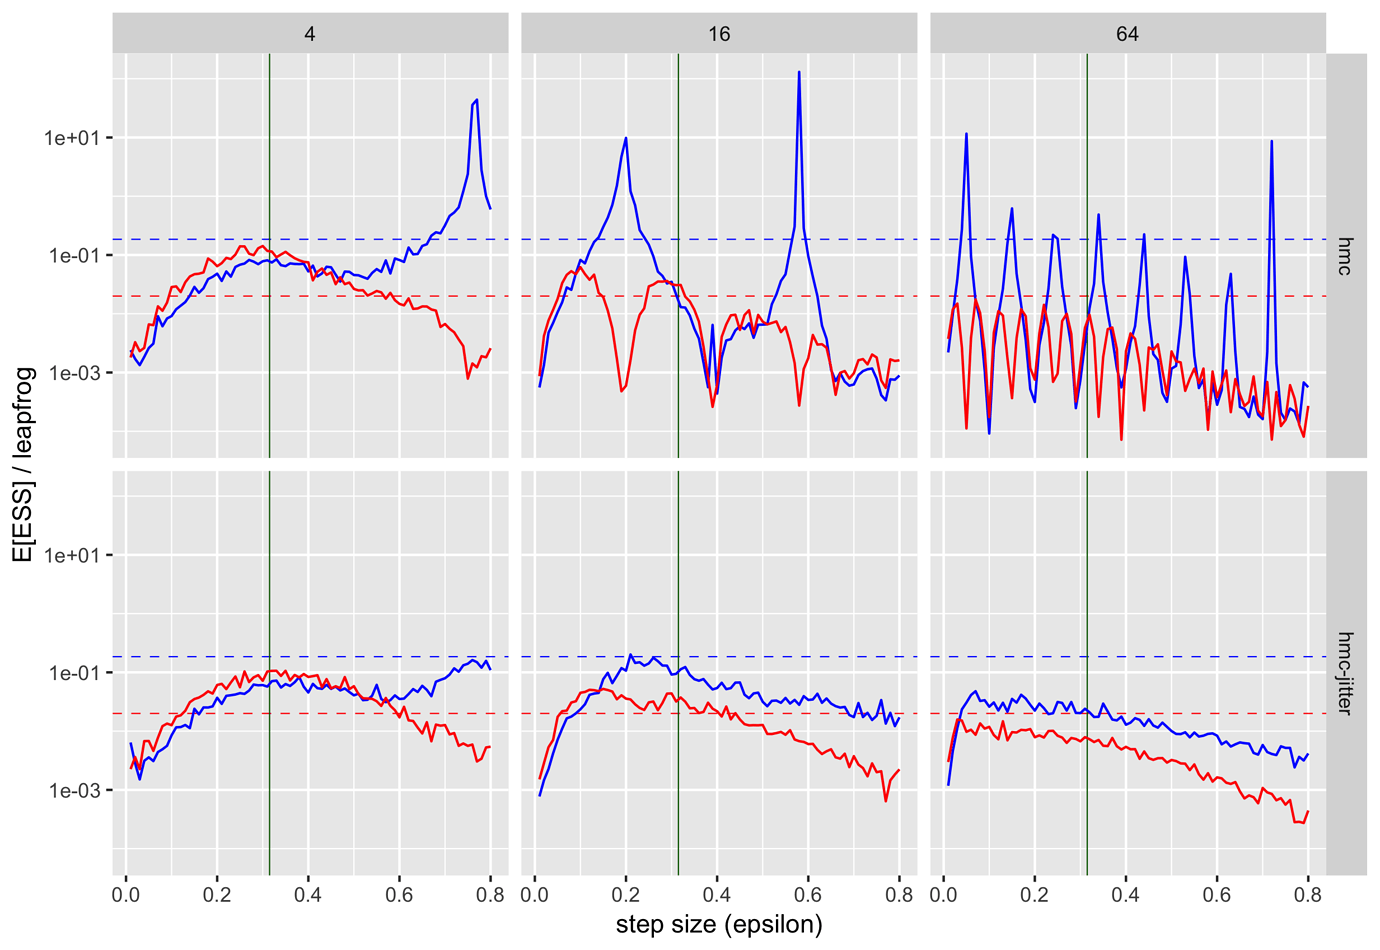
\includegraphics[width=2.6in]{img/hmc-harmonics.png}
\end{center}

\sld{A solution framework: Gibbs self tuning (GIST)}
\begin{itemize}
\item \myemph{Couple tuning parameters} $\alpha$ (step
  size, number of steps, mass matrix)
\item \myemph{Free choice} of conditional tuning-parameter distribution $p(\alpha \mid \theta, \rho)$
\item Each iteration, \myemph{Gibbs sample} $\alpha^* \sim p( \cdot \mid \theta,
  \rho)$
\item Conditionally propose $\theta^*, \rho^* = \Phi^{T^*}_{\epsilon^*,
    \Sigma^*}(\theta, \rho)$ given $\alpha^* = \epsilon^*,
  \Sigma^*, T^*$
\item Metropolis-Hastings (within Gibbs) \myemph{accept probability} for proposal $\theta^*,
  \rho^*$ is
  $$
  1 \wedge
  \frac{p(\theta^*, \rho^*)}
  {p(\theta, \rho)}
  \cdot
  \frac{p(\alpha^* \mid \theta^*, \rho^*)}
       {p(\alpha^* \mid \theta, \rho)}
       $$
\item Includes randomized step size or steps HMC, multinomial HMC,
  NUTS, apogee-to-apogee, plus \myemph{exciting new options}
\end{itemize}

\sld{Randomized HMC is GIST}
\begin{itemize}
\item HMC works with \myemph{randomized tuning} (e.g., steps $L$ or
  step size $\epsilon$)
\item Other tuning parameters are fixed (i.e., delta function distributions)
\item \myemph{Randomizing} step size or number of steps \myemph{removes
    harmonics} that plague HMC with fixed step size and steps, e.g.,
  $$p(L \mid \theta, \rho) = \textrm{uniform}(L \mid 1, N).$$
\item If tuning parameter distribution does \myemph{not depend on position or
  momentum}, then $p(\alpha^* \mid \theta, \rho) = p(\alpha^* \mid \theta^*,
  \rho^*)$, and thus
  $$
  1 \wedge
  \frac{p(\theta^*, \rho^*)}
       {p(\theta, \rho)}
  \cdot
  \frac{p(\alpha^* \mid \theta^*, \rho^*)}
       {p(\alpha^* \mid \theta, \rho)}
       =
       1 \wedge
       \frac{p(\theta^*, \rho^*)}{p(\theta, \rho)}
  $$       
\end{itemize}

\sld{Multinomial HMC is a GIST sampler}
\begin{itemize}
\item Multinomial HMC fixes a \myemph{maximum number of steps} $L$, step size
  $\epsilon$, and mass matrix $\Sigma$.
\item Each iteration, take $F \sim \textrm{uniform}(0, L)$ \myemph{forward
    steps} and $B = L - F$ \myemph{backward steps}.
  \begin{subitemize}
  \item Let $\Phi^{-t}_{\epsilon, \Sigma}(\rho, \tau)
    = \Phi^{t}_{\epsilon, \Sigma}(\rho, -\tau)$ (i.e., \myemph{flip
      momentum})
    \end{subitemize}
  \item \myemph{Generate number of steps} with probability
    $$p(t) \propto p(\theta(t), \rho(t))$$ from
    candidates  $\theta(t), \rho(t) = \Phi^t_{\epsilon,
      \Sigma}(\theta, \rho)$, where $t \in \{ -B, -B + 1, \ldots, 0, 1, \ldots, F \}$
\item The GIST \myemph{acceptance probability is 100\%}!
\end{itemize}

\sld{Proof of multinomial 100\% acceptance}
\begin{itemize}
\item Without loss of generality, \myemph{assume} $F + B = L$ and selected $n > 0$
\item GIST \myemph{acceptance probability} is
  $\frac{p(\theta(n),\,   \rho(n))}
        {p(\pos{\theta}{0},\, \pos{\rho}{0})}
   \cdot
   \frac{p(n \, \mid \, \theta(n),\, -\rho(n))}
        {p(n \, \mid \, \pos{\theta}{0},\, \pos{\rho}{0})}$
      \item Length $L$ trajectories (forward and backward in time) from 0 to $n$ are same
        as from $n$ to 0, so \myemph{same denominator} (see next slide)
        \begin{subitemize}
          \item $p(n \mid \pos{\theta}{0}, \pos{\rho}{0}) = \sum_{i=L-n}^0 
  \frac{p(\theta(n),\, \rho(n))}
  {\sum_{j=i}^{i + L} p(\theta(j),\, \rho(j))}$
\item  $p(n \mid \theta(n),\, -\rho(n)) = \sum_{i=L-n}^0 
  \frac{p(\pos{\theta}{0},\, \pos{\rho}{0})}
  {\sum_{j=i}^{i + L} p(\theta(j),\, \rho(j))}$
\end{subitemize}
\item The \myemph{correction} for detailed balance reduces to
$\frac{p(n \, \mid \, \theta(n),\, -\rho(n))}
      {p(n \, \mid \, \theta(n),\, \rho(n))}
      = \frac{p(\pos{\theta}{0},\, \pos{\rho}{0})}
      {p(\theta(n),\, \rho(n))}$
\item Thus \myemph{acceptance is 100\%}.
\end{itemize}

\sld{Multinomial path similarity illustration}
\begin{itemize}
\item Trajectories \myemph{starting at $0$} and \myemph{including $N$}
\end{itemize}
\begin{verbatim}
     F = L,   B = 0:             0 ... N ...        L

     F = L-1, B = 1:          -1 0 ... N ... (L-1)

        .                           .
        .                           .
        .                           .

     F = N, B = L-N:  -(L-N) ... 0 ... N
\end{verbatim}
\begin{itemize}
\item are \myemph{identical} to trajectories \myemph{starting at $N$}
  and \myemph{including $0$} (flip F \& B)
\end{itemize}

\sld{NUTS, AAPS, and autoMALA are GIST samplers}
\begin{itemize}
\item The \myemph{no-U-turn sampler} (NUTS) is a GIST sampler.
\item The \myemph{apogee-to-apogee path
    sampler} (AAPS) is a GIST sampler.
\item The \myemph{autoMALA sampler} is a GIST sampler.
\item Cast both as conditional \myemph{distributions on number of steps} given
  current position and momentum with a \myemph{multinomial acceptance}.
\item There are detailed \myemph{proofs in the paper}.
\end{itemize}

\sld{U-turn condition}
\begin{itemize}
\item We developed a new sampler based on NUTS's \myemph{U-turn condition}:
$$U(\pos{\theta}{0}, \pos{\rho}{0}) = \textrm{arg min}_t  (\pos{\theta}{t} -
  \pos{\theta}{0})^{\top} \cdot \pos{\rho}{t} < 0$$
\begin{center}
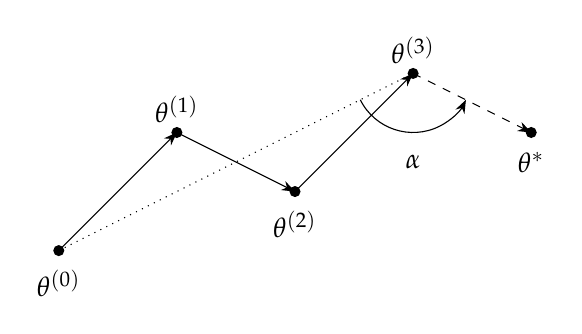
\begin{tikzpicture}[>=Stealth]
  % Define points along the arc
  \coordinate (A) at (0,0);
  \coordinate (B) at (1.5,1.5);
  \coordinate (C) at (3,0.75);
  \coordinate (D) at (4.5,2.25); % Second to last point
  \coordinate (E) at (6,1.5); % Last point

  \node at (A) [below=0.125cm] {$\pos{\theta}{0}$};
  \node at (B) [above=0cm] {$\pos{\theta}{1}$};
  \node at (C) [below=0.125cm] {$\pos{\theta}{2}$};
  \node at (D) [above=0cm] {$\pos{\theta}{3}$};
  \node at (E) [below=0.125cm] {$\theta^*$};

  % Draw trajectory with arrows
  \draw[->] (A) -- (B);
  \draw[->] (B) -- (C);
  \draw[->] (C) -- (D);
  \draw[->,style=dashed] (D) -- (E);

  % Place solid circles at discretized positions
  \foreach \point in {A,B,C,D,E}
    \fill (\point) circle (2pt);

  % Dotted line from first to second to last point
  \draw[dotted] (A) -- (D);

  % Auxiliary point for angle calculation
  % This creates an invisible point extending the dotted line beyond 'D' for angle drawing
  \coordinate (F) at ($(A)!-1.2!(D)$); % Extend line beyond D for angle marking

  % Arc for angle indication
  \pic[draw, ->, "$\alpha$", angle eccentricity=1.5, angle radius=0.75cm] {angle = F--D--E};
\end{tikzpicture}
\end{center}
\end{itemize}

\sld{Number of steps proposal}
\begin{itemize}
  \item Non-zero steps distributed \myemph{uniformly up to U-turn}
$$p(n \mid \pos{\theta}{0}, \pos{\rho}{0}) = \textrm{uniform}(n \mid 1, N),$$
where $N = U(\pos{\theta}{0}, \pos{\rho}{0}) - 1$
    \begin{subitemize}
    \item \myemph{excludes initial} point and \myemph{excludes U-turn} point
    \item unlike multinomial, (revised multinomial) NUTS, and AAPS, only \myemph{proposes forward in time}
    \end{subitemize}
\end{itemize}

% where $(\pos{\theta}{n}\!, \pos{\rho}{n}) = \Phi_h^n(\theta, \rho)$. 

\sld{Sketch of leapfrogs per iteration (still go back)}
  \begin{center}
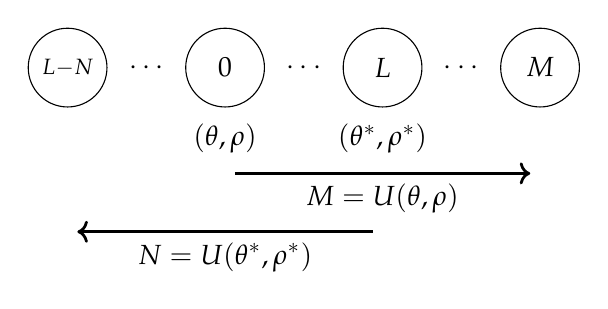
\begin{tikzpicture}[node distance=1cm and 0.5cm]
    % Top row nodes
    \node[circle,draw,minimum size=1cm] (LM) {\footnotesize $L{-}N$};
    \node[minimum size=1cm,right of=LM] (dots1) {$\cdots$};
    \node[circle,draw,minimum size=1cm,right of=dots1] (0) {$0$};
    \node[minimum size=1cm,right of=0] (dots2) {$\cdots$};
    \node[circle,draw,minimum size=1cm,right of=dots2] (L) {$L$};
    \node[minimum size=1cm,right of=L] (dots3) {$\cdots$};
    \node[circle,draw,minimum size=1cm,right of=dots3] (N) {$M$};
    
    % 2nd row nodes
    \node[below = 0.05cm of LM] (n_a1) {$\strut$};
    \node[below = 0.05cm of 0] (theta_rho) {$\strut (\theta, \rho)$};
    \node[below = 0.05cm of L] (theta_rho_star) {$\strut (\theta^*, \rho^*)$};
    \node[below = 0.05cm of N] (n_a2) {$\strut$};

    
    % 3rd row arrow
    \node[below = -0.25cm of n_a1] (n_a3) {$\strut$};
    \node[below = -0.25cm of theta_rho] (start_arrow2) {$\strut$};
    \node[below = -0.25cm of theta_rho_star] (n_a4) {$\strut$};
    \node[below = -0.25cm  of n_a2] (end_arrow2) {$\strut$};
    \draw[->, line width=1pt] (start_arrow2) -- (end_arrow2) node[midway, below] {$M = U(\theta, \rho)$};
    
    % 4th row arrow
    \node[below = 0.05cm of n_a4] (start_arrow1) {$\strut$};
    \node[below = 0.05cm of n_a3] (end_arrow1) {$\strut$};
    \draw[->, line width=1pt] (start_arrow1) -- (end_arrow1) node[midway, below] {$N = U(\theta^*, \rho^*)$};
\end{tikzpicture}
\end{center}
\vspace*{-8pt}
\begin{subitemize}
\item $M$ leapfrogs \myemph{from initial} $\theta, \rho$ to U-turn; $p(L \mid
  \theta, \rho) = \textrm{uniform}(L \mid 1, M)$;
  % $\theta^*, \rho^* = \Phi^{L}_{\epsilon, \Sigma}(\theta, \rho)$
\item $N$ leapfrogs \myemph{from proposal} $\theta^*, -\rho^*$ to U-turn; $p(L
  \mid \theta^*, -\rho^*) = \textrm{uniform}(L \mid 1, N)$
\item \myemph{Metropolis-Hastings accept}: $\frac{\displaystyle p(\theta^*, -\rho^*) \cdot \textrm{uniform}(L \mid
    1, M)}{\displaystyle p(\theta, \rho) \cdot
    \textrm{uniform}(L \mid 1, N)}
  = \frac{\displaystyle p(\theta^*, -\rho^*) \cdot N}
  {\displaystyle p(\theta, \rho) \cdot M}$
\end{subitemize}

\sld{Acceptance probability breakdown}
\begin{itemize}
\item \myemph{Metropolis-Hastings}: $\frac{\displaystyle p(\theta^*, -\rho^*) \cdot \textrm{uniform}(L \mid
    1, M)}{\displaystyle p(\theta, \rho) \cdot
    \textrm{uniform}(L \mid 1, N)}
  = \frac{\displaystyle p(\theta^*, -\rho^*) \cdot N}
  {\displaystyle p(\theta, \rho) \cdot M}$
\item Ratio of $p(\theta^*, \rho^*) / p(\theta, \rho) = 1$ if
  \myemph{Hamiltonian dynamics perfect}
  \begin{subitemize}
  \item will vary with leapfrog
  \item \myemph{most steps} $< 1$ with decently large step size
  \end{subitemize}
\item Ratio of $N / M$ depends on how balanced U-turns are
  \begin{subitemize}
    \item very well behaved with constant curvature (e.g., w.\ std.\
      normal, $M \approx N$)
    \item more variable with varying curvature (i.e, non-constant log
      density Hessian)
    \end{subitemize}
\end{itemize}

\sld{``Learning curve'' unit test}
\begin{itemize}
\item I like to plot \myemph{estimation error} for $\mathbb{E}[\theta]$ and
  $\mathbb{E}[\theta^2]$ for \myemph{{\slshape\bfseries long}\, chains}.
% \item For example, standard \myemph{HMC asymptotes on funnels} as it can't 
% sample multiscale well. 
\item \myemph{1M iterations} of 100D std.\ normal; \myemph{dashed is
    CLT} $\textrm{se} = \textrm{sd} / \sqrt{N}$.
\end{itemize}
\begin{center}
  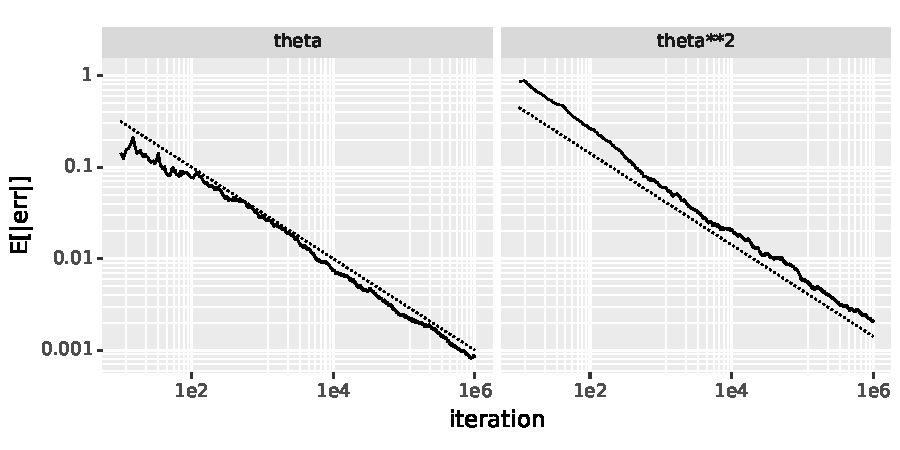
\includegraphics[width=3in]{img/learning_curve_uniform_full_100D.pdf}
\end{center}

\sld{Encouraging longer jumps}
\begin{itemize}
\item Simple GIST generalizes to \myemph{initial exclusion fraction} $\psi \in 
    (0, 1)$:
$$p(n \mid \pos{\theta}{0}, \pos{\rho}{0}) = \textrm{uniform}(n \mid 
1 \vee \lceil \psi \cdot  N \rceil, \ N).$$
\item Must balance \myemph{longer accepted paths} with \myemph{more rejections} from \myemph{irreversibility}
  (zero return probability)
\item \myemph{AAPS} biases \myemph{longer jumps} using clever weighting
  (e.g., MSJD).
  \begin{subitemize}
%    \item Sam Livingstone pointed out AAPS; always \myemph{talk to everyone}
    \item GIST compatible, so \myemph{our engineers} (i.e., me) are evaluating
    \end{subitemize}
\item Revised \myemph{NUTS} (Betancourt 2017) 
  biases by \myemph{up-weighting second half}.
\end{itemize}

\sld{Evaluation metrics}
\begin{itemize}
\item Number of \myemph{leapfrog steps} (lower is better)
\item \myemph{Mean square jump distance} (MSJD) (higher is better for
  $\mathbb{E}[\theta]$)
\begin{subitemize}
\item $\displaystyle \textrm{MSJD} = \textrm{mean}_{i < N} \,
  \left(\pos{\theta}{i + 1} - \pos{\theta}{i}\right)^2$ \hfill (inversely
  related to lag-1 autocorr)
\end{subitemize}
\item \myemph{No return} is number of irreversible paths due to
  \myemph{premature U-turns} (including path fraction).
\item \myemph{Reject} is total Metropolis-Hastings rejections
  \begin{subitemize}
    \item includes rejections due to no return and low accept
      probability
    \end{subitemize}
\item Standardized \myemph{Root mean square error} in estimation of
  $\mathbb{E}[\theta]$ and $\mathbb{E}[\theta^2]$
  \begin{subitemize}
  \item root matches \myemph{units} of parameters; standardizing
    reduces to \myemph{$Z$-scores}
  \end{subitemize}
\end{itemize}

\sld{How does it work?\hfill (500 dim std.\ normal)}
\vspace*{-9pt}
\begin{center}
  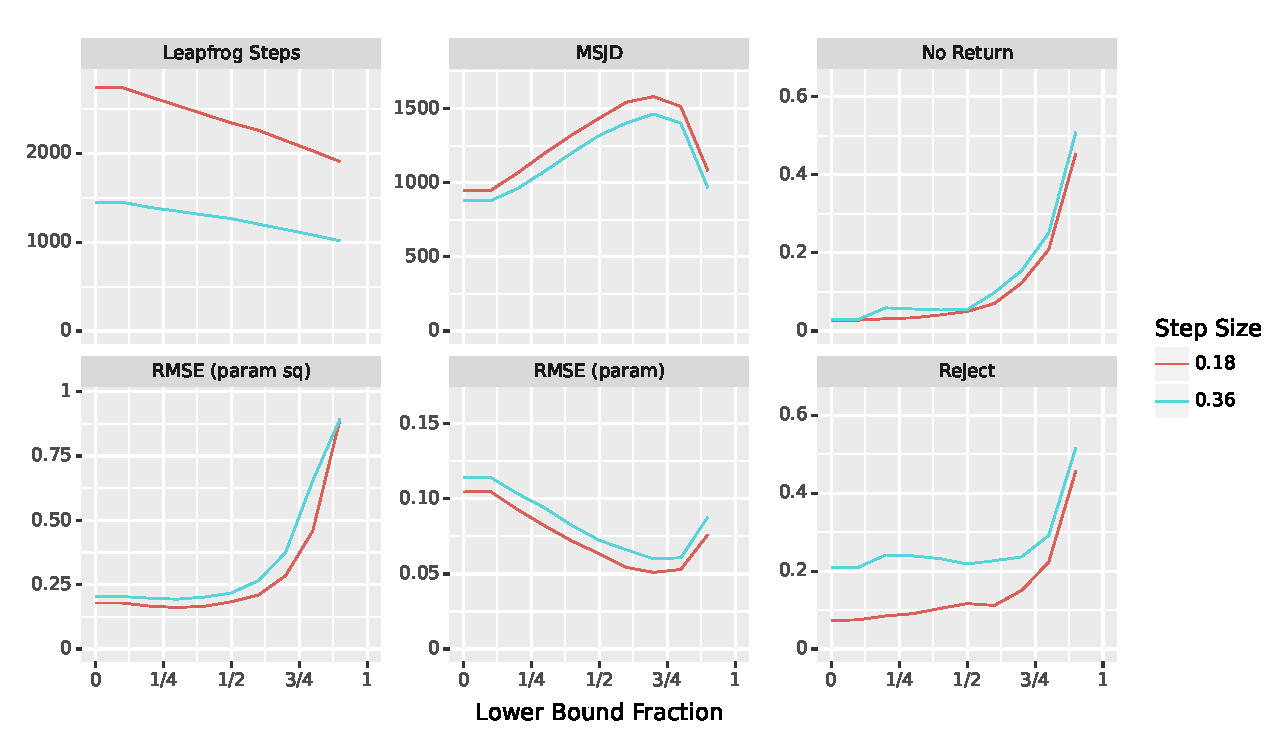
\includegraphics[width=3.9in]{img/uniform_prob_steps_plot.pdf}
\end{center}

\sld{RMSE for parameter estimates (lower better)}
\vspace*{-9pt}
\begin{center}
  \includegraphics[width=0.95\textwidth]{img/vs_NUTS_rmse_param.pdf}
\end{center}

\sld{RMSE for squared parameter est.\ (lower better)}
\vspace*{-9pt}
\begin{center}
  \includegraphics[width=0.95\textwidth]{img/vs_NUTS_rmse_param_sq.pdf}
\end{center}

\sld{MSJD (higher better for $\mathbb{E}[\theta]$)}
\vspace*{-9pt}
\begin{center}
  \includegraphics[width=0.95\textwidth]{img/vs_NUTS_MSJD.pdf}
\end{center}

\sld{Leapfrog steps (lower better)}
\vspace*{-9pt}
\begin{center}
  \includegraphics[width=0.95\textwidth]{img/vs_NUTS_Leapfrog_Steps.pdf}
\end{center}

\sld{Neal's funnel and varying curvature}
\begin{itemize}
\item \myemph{Neal's funnel} has really \myemph{nasty varying curvature}:
$$
    x \sim \textrm{normal}(0, 3)
\qquad
y_{1:D-1} \sim \textrm{normal}(0, \exp(\alpha_1 / 2))
$$
\item \myemph{Terrible condition} in neck \myemph{and} mouth w. \myemph{rotated eigenvectors}
\item Hamiltonian Monte Carlo with any \myemph{fixed step size fails}
  (e.g., NUTS)
\end{itemize}
\begin{center}
  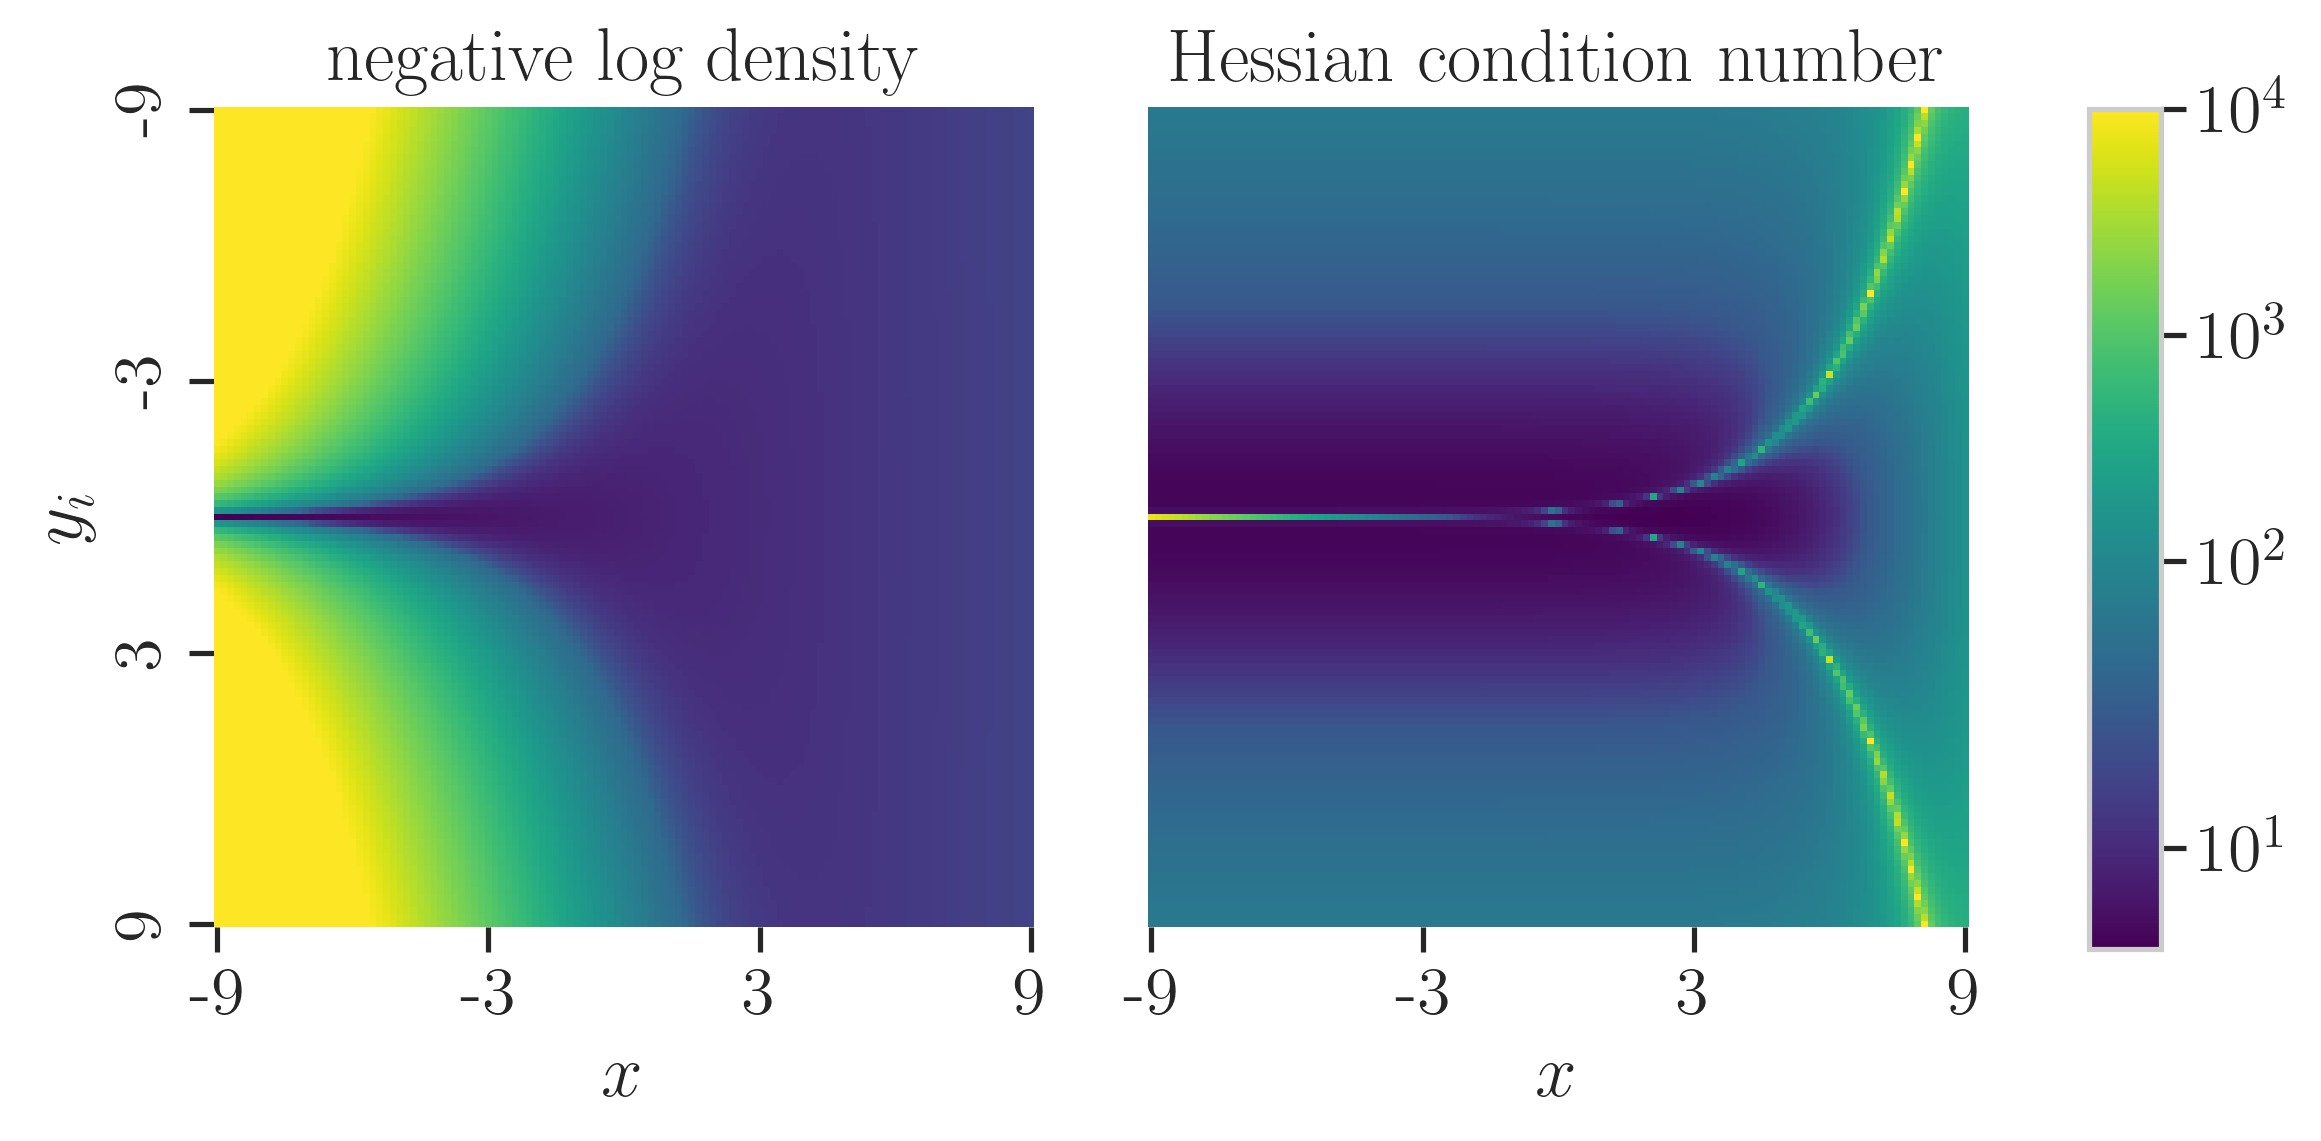
\includegraphics[width=2.25in]{img/funnel_density_hessian.png}
\end{center}
  
\sld{Alternative: delayed rejection HMC}
\begin{itemize}
\item I've been working on this problem for \myemph{three years}
\item \myemph{Delayed rejection HMC} w. Chirag
  Modi, Alex Barnett ({\slshape Bayesian Analysis})
  \begin{subitemize}
  \item if proposal \myemph{fails, try again} with smaller step size
  \item requires matching ``ghost proposals'' for balance, which are \myemph{costly}
    \end{subitemize}
\item \myemph{Delayed rejection generalized HMC} w.\ Gilad
      Turok, Chirag Modi ({\slshape NeurIPS} submission)
    \item \myemph{DR works}, but \myemph{costly and complicated} and not clear how
      to generalize.
    \item G-HMC \myemph{tunes locally}
      \item Chirag's exploring \myemph{combining GIST
      \& DR-G-HMC}
\end{itemize}

\sld{Tuning step size with GIST}
\begin{itemize}
\item \myemph{Fix} integration time $T \in (0, \infty)$, mass matrix $\Sigma$
\item \myemph{Each iteration}, \myemph{find minimum} $N \in \{ 1, 2, 3, 4, 6, 
  8, 11, 16, 22, 32, \ldots \}$ (i.e., $\sqrt{2}^n$) s.t. with $N$ leapfrog 
  steps of size $\epsilon = T / N$, Hamiltonian \myemph{error is bounded}
  to accept probability $ > p$
  $$
  N = \textrm{arg min}_n \ H^{\textrm{max}} - H^{\textrm{min}} > \log p, 
  $$
  where 
  $$
  H^{\textrm{max}} = \textrm{arg max}_n \ H \circ \Phi^{n}_{\epsilon,\Sigma}(\pos{\theta}{n}, \pos{\rho}{n}) 
  $$
  $$
  H^{\textrm{min}} = \textrm{arg min}_n \ H \circ \Phi^{n}_{\epsilon,\Sigma}(\pos{\theta}{n}, \pos{\rho}{n}) 
  $$
\item \myemph{Sample step size} $N \sim \textrm{poisson}(L)$ \hfill (perhaps use
  more dispersed?)
\end{itemize}

\sld{Step size and number of steps adaptation?}
\begin{itemize}
\item Idea: set \myemph{step size in outer loop} and \myemph{number of steps} in
  inner loop, then randomize
  \begin{subitemize}
    \item i.e., find max stepsize $\epsilon$ such that trajectory to
      U-turn has bounded error
  \end{subitemize}
\item Nawaf Bou-Rabee has a \myemph{prototype implementation} and it \myemph{appears to work}
\end{itemize}

\sld{GIST fits the tails of the funnel}
\begin{itemize}
\item Here's a \myemph{histogram of 20K draws} of log scale ($y$); marginal is $\textrm{normal}(0, 3)$
\end{itemize}
\begin{center}
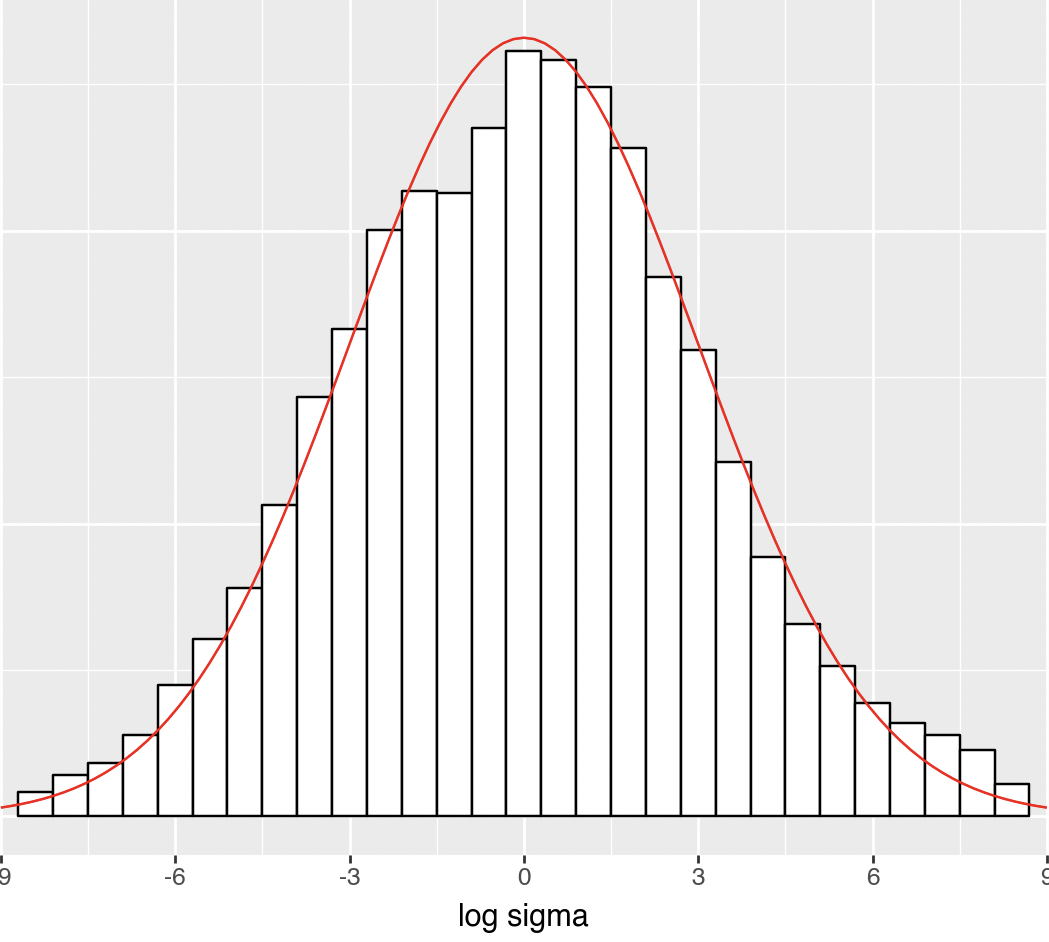
\includegraphics[width=1.5in]{img/funnel-step-size-GIST.png}
\end{center}
\begin{itemize}
\item Learning curve \myemph{unit tests pass}
\item 1M iteration histogram \myemph{looks perfect} ($\chi$ by eye)
\end{itemize}

\sld{Mass matrix adaptation?}
\begin{itemize}
\item Use a local (negative inverse) Hessian estimate $M$ as local 
  mass matrix 
\begin{subitemize}
\item perfect pre-conditioner with multivariate normal 
\end{subitemize}
\item Randomization: $\Sigma \sim \textrm{invWishart}(M, \nu)$
\begin{subitemize}
\item $\nu$ controls concentration around $M$ and hence reversibility 
\end{subitemize}
\item Trick will be making this \myemph{``implicit''} to use more than
  initial position.
\item \myemph{Haven't evaluated} yet. 
\end{itemize}

\sld{What's next}
\begin{itemize}
\item \myemph{One GIST sampler to rule them all}, which
\begin{subitemize}
\item locally adapts \myemph{step size} (stability condition)
\item locally adapts \myemph{number of steps} (no-U-turn condition)
\item locally adapts \myemph{mass matrix} (wide open)
\item uses \myemph{generalized HMC} (for per-step adaptation) 
\end{subitemize}
\end{itemize}
  
\sld{\textit{arXiv} paper;\, public GitHub}
\begin{itemize}
\item Nawaf Bou-Rabee, Milo Marsden, and Bob Carpenter. 2024. \myemph{GIST: Gibbs
self-tuning for locally adaptive Hamiltonian Monte
Carlo}. \textit{arXiv} 2404.15253.
\item GitHub: \texttt{https://github.com/bob-carpenter/\myemph{adaptive-hmc}}
\vfill
\item We would \myemph{appreciate feedback} on paper and
  Python code \myemph{before journal submission}.
\end{itemize}
\end{document}


